\usetikzlibrary{shapes,arrows}
\tikzstyle{block} = [draw, fill=blue!20, rectangle, 
    minimum height=2em, minimum width=4em]
\tikzstyle{circle} = [draw, fill=blue!20, ellipse, 
    minimum height=2em, minimum width=2em]
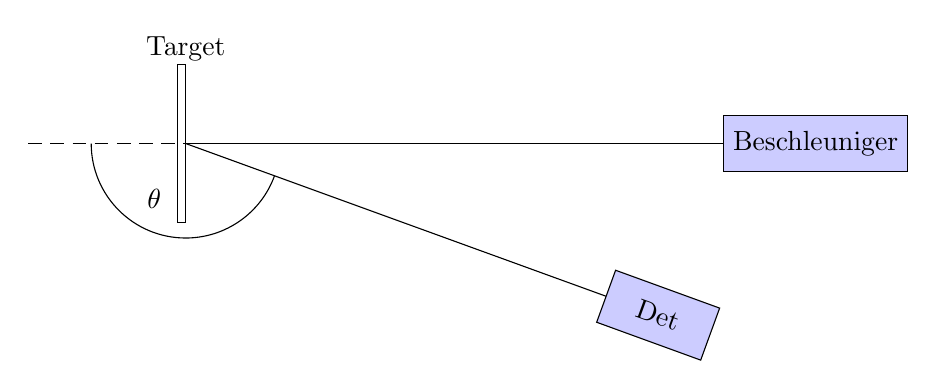
\begin{tikzpicture}
 \coordinate (L) at (-5,0);
 \coordinate (R) at (5,0);
\coordinate (B) at (-3,0);
\coordinate (A) at (3,-2.18);
\coordinate (O) at (0,0);

\draw[dash pattern=on5pt off3pt] (L) -- (R);
\draw[dash pattern=on5pt off0pt] (A) -- (B);
\draw[dash pattern=on5pt off0pt] (R) -- (B);

\draw (-4.2,0) arc (180:340:1.2);
\draw (-3,-1) rectangle (-3.1,1);

\node[] at (-3.4,-0.7)  {$\theta$};
\node[] at (-3,1.2)  {Target};


\node[block, name=det2, rotate=-20] at (A) {Det};
\node[block, name=Beschleuniger, rotate=0] at (R) {Beschleuniger};

\ ;\end{tikzpicture}